\labday{4 April 2023}

\experiment{MAZ04}

\textbf{UCASS-AA-MAZ04-001 continued:}

It was decided, in order to rule out firmware or software issues, that the UCASS could be triggered using the fibre LED to view output counts. The laser turned itself off, but was reactivated when the unit was power-cycled. Blue-tac was positioned over the beamstop, the lights were switched off. The frequency of the pulse-generator was set to \SI{10}{\hertz} for 10 particles per second, the pulse width to \SI{10}{\micro\second}, and the ampitude to \SI{1}{\volt}---enough to activate the LED but not saturate the TIA. The setup is pictured in Fig. \ref{fig:UCASSFibreRig}. There were no couts observed, which indicates that the problem lies in the electronics as opposed to the alignment. This was conducive to the results of the fibre measurement. Inspection of the unit confirmed that one of the opamps responsible for DC-restoration was not attached properly, which was due to bad soldering. The chip was soldered on properly, and the other opamps were checked for defects (one other was found), I now believe this is what was wrong with 011 and will check the board again before removing the mirror. The unit now draws the correct amount of current. \textbf{Counts are now registered at \SI{1179}{ADC} for an input of \SI{900}{\milli\volt}}. The device now works properly with sample aerosol.

\begin{figure}[H]
\begin{center}
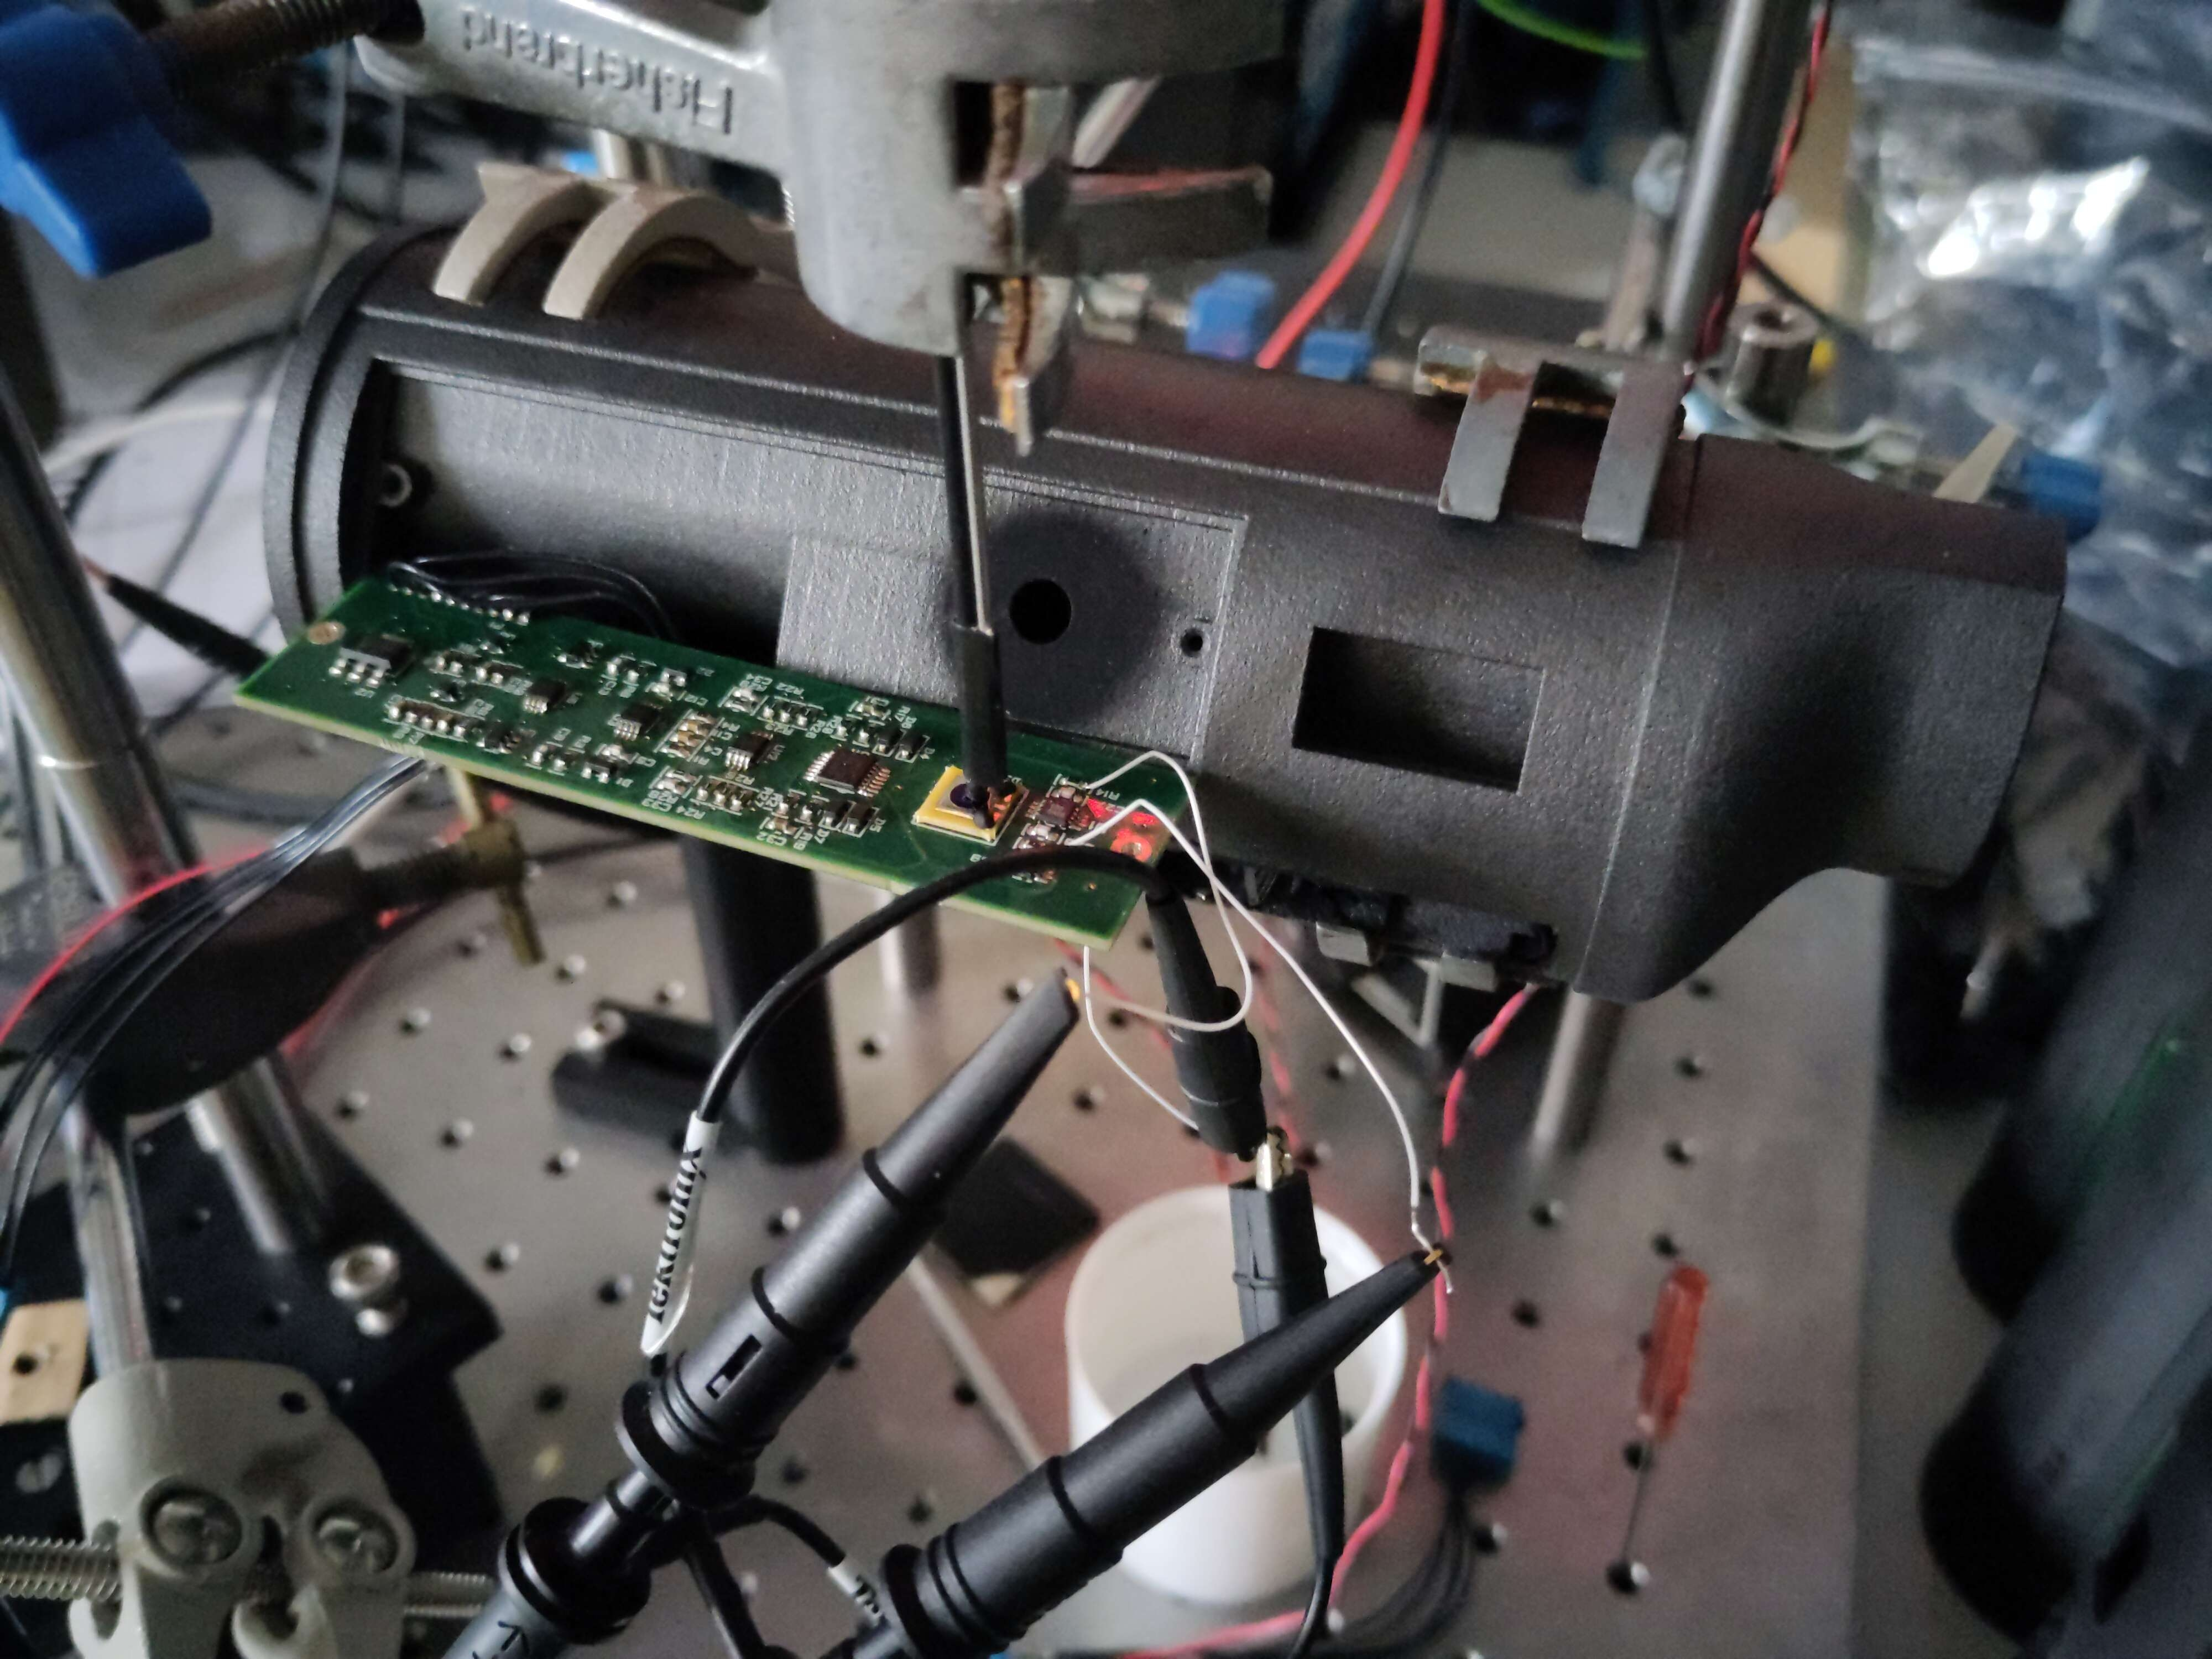
\includegraphics[width=0.5\linewidth]{Figures/UCASSFibreRig}
\end{center}
\caption{Fibre test setup for UCASS.}
\label{fig:UCASSFibreRig}
\end{figure}

\textbf{UCASS-AD-MAZ04-011 continued:}

The above procedure was repeated for the 011 unit. One of the opamps was disconnected from the board in two places. The unit now draws the correct current. The height of the pulse was adjusted to \SI{1.2}{\volt} to account for the different gain. \textbf{This produced a value of approximately 1200}, but it was visibly more broad than the aerosol board; this points to gain instability in this configuration. The unit now produced counts when fitted together and tested with spray.

\textbf{UCASS-AA-MAZ04-006:}

There was a visible short on one of the opamps, which would explain why the unit was drawing too much current. Once the opamp was resoldered, the unit drew a normal amount of current. On the pulse generator, a gain of \SI{900}{\milli\volt} was used, and the unit performed as expected, with pulses in the 2100 region, and much narrower than the droplet UCASS. It was long suspected that the droplet gain suffers from instability, but the test did not exist to prove this since aerosol distributions can be broad (even so-called monodisperse ones). \textbf{The unit now performs as expected with test aerosol}.

\textbf{UCASS-AD-MAZ04-009:}

One of the opamp pins was not connected, and one opamp apeared to be twisted (althoguh not so bad that it would cause a short). These issues were rectified; the unit draws the correct current (\SI{125}{\milli\ampere}. When connected to the pulse-generator, there are still no counts shown on the software, despite the TIA outputs appearing reasonable.



\experiment{MPICCE}

\begin{itemize}
\item Instruments shipped by the end of April (first deadline).
\item 2 types in-situ and vertical sampling.
\item PVM and fog-monitor.
\item A DMT instrument will be in the chamber. SHIFAS-DPOL (i think).
\item There is a PPD-2K which will be part of the campaign, potentially my participation is now pointless.
\item People need to update Ottmar on their own technical details.
\item No aim for expansion cloud.
\item Anything in the chamber will require at least 4m long cables.
\item Two nozzels to alternate between water and ice clouds, to study the transition.
\item Can form different ice crystal habits still.
\item Cables through KF40 flange and sealed (for instruments in the chamber).
\item Instruments in the chamber will be sealed for the duration of the campaign.
\item Concerns about super-cooled water, but this may not be justified.
\item \SI{80}{\cubic\metre} chamber.
\item More chance of secondary crystals with sray clouds.
\end{itemize}



